% Este archivo es parte de la memoria del proyecto fin de carrera
% de Aarón Bueno Villares. Protegida bajo la licencia GFDL.
% Para más información, la licencia completa viene incluida en el
% fichero fdl-1.3.tex
%
% Fuente tomada del PFC 'DSMemorizer' de Diego Barrios Romero, a su vez
% tomada del PFC 'libgann' de Francisco Javier Vázquez Púa, a su vez tomada de la plantilla LaTeX para
% la realización de Proyectos Final de Carrera de Pablo Recio Quijano.

% Copyright (C) 2008 Francisco Javier Vázquez Púa
% Copyright (C) 2009 Pablo Recio Quijano
% Copyright (C) 2009 Diego Barrios Romero

% Copyright (C) 2009 Aarón Bueno Villares

\begin{center}

\Large{\textbf{\fpt}} \\
\vspace{.5cm}
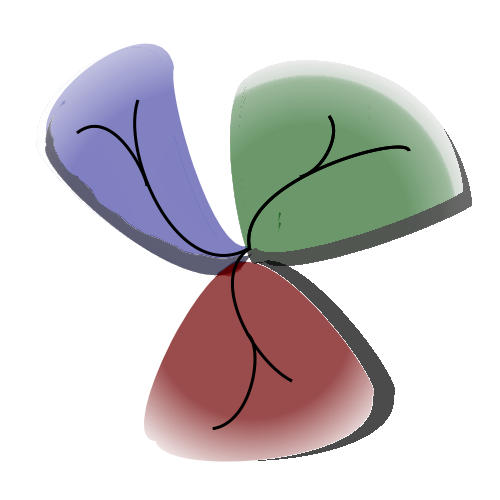
\includegraphics[scale=.2]{../../Resources/logo.png}
\vspace{.5cm}

\Large{\textbf{Software de visualización de árboles filogenéticos}} \\

\vspace{1cm}

\huge{\textbf{\underline{Memoria del proyecto}}} \\

\vspace{0.5cm}

\tiny{Aarón Bueno Villares} \\

\vspace{0.5cm}

\end{center}

\tableofcontents

\vspace{12cm}

\begin{center}
\begin{minipage}{15cm}
\rule{15cm}{.3pt}
\\
\tiny{
Este documento ha sido liberado bajo Licencia GFDL 1.3 (GNU Free
Documentation License).\\

Copyright (c) 2010 Aarón Bueno Villares.\\

Permission is granted to copy, distribute and/or modify this document
under the terms of the GNU Free Documentation License, Version 1.3 or
any later version published by the Free Software Foundation; with no
Invariant Sections, no Front-Cover Texts, and no Back-Cover Texts. A
copy of the license is included in the section entitled "GNU Free
Documentation License".
}
\rule{15cm}{.3pt}
\end{minipage}
\end{center}
